% The "zoo" of vector-calculus integrals organized by dimension, with
% grad/curl/div/scalar-curl relating them; grand summary of the chapter.
% Source: book/tex/diffgeo/stokes.tex (§ Stokes' theorem in general).
\documentclass[border=3mm]{standalone}
\usepackage{amsmath,amssymb}\usepackage{tikz}\usetikzlibrary{arrows.meta}
\newcommand{\dx}{\,\mathrm{d}x}\newcommand{\dt}{\,\mathrm{d}t}
\newcommand{\du}{\,\mathrm{d}u}\newcommand{\dv}{\,\mathrm{d}v}
\newcommand{\rr}{\mathbf r}\newcommand{\FF}{\mathbf F}
\begin{document}
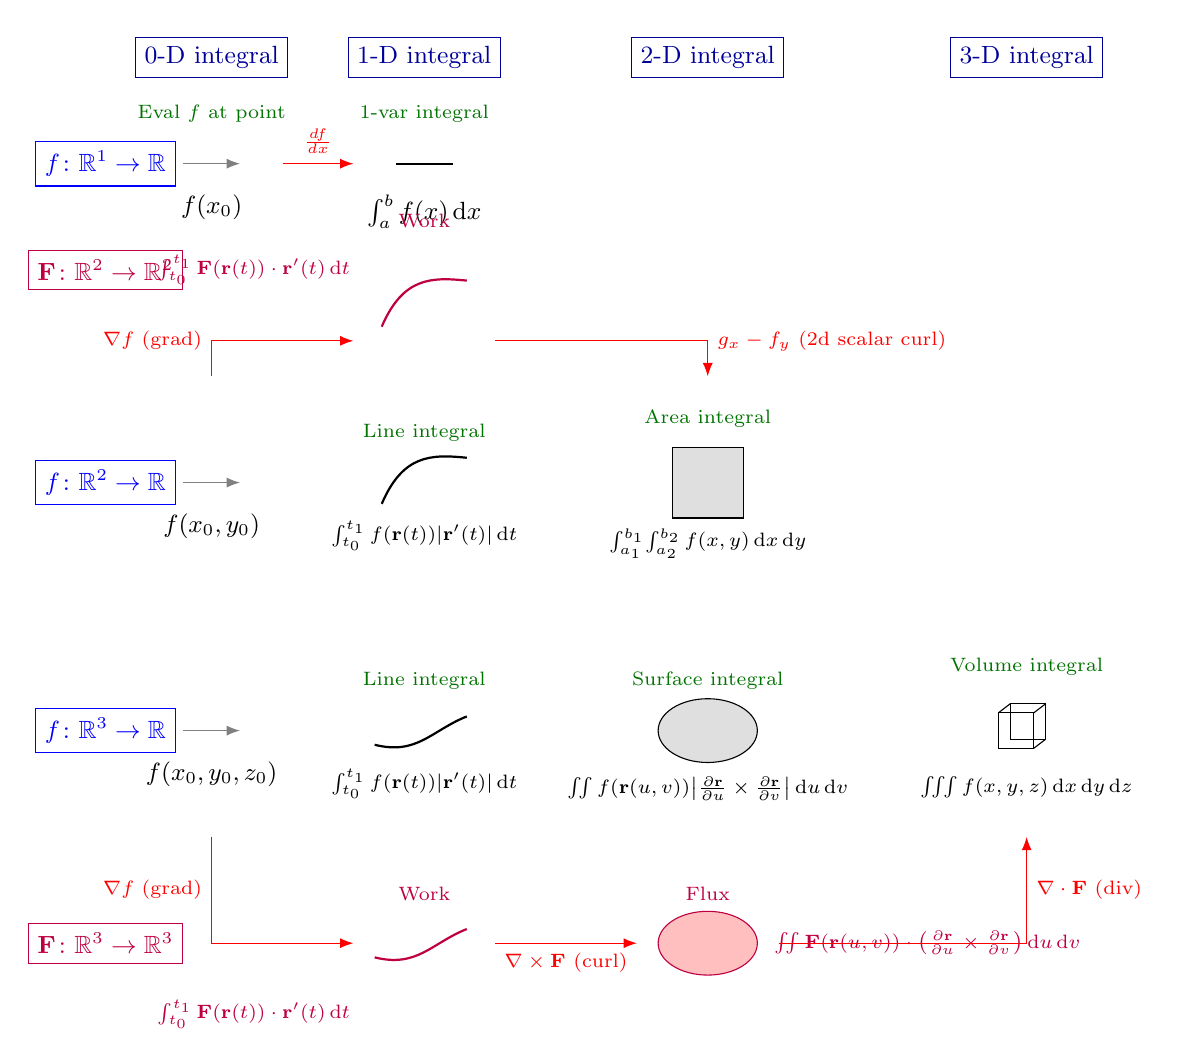
\begin{tikzpicture}[scale=0.9,font=\small,>={Latex},
   ax/.style={gray,-{Latex}},
   ig/.style={red}, blu/.style={purple}]
  % type boxes
  \node[draw,blue] at (-0.5,8){$f\colon\mathbb R^1\to\mathbb R$};
  \node[draw,purple] at (-0.5,6.5){$\FF\colon\mathbb R^2\to\mathbb R^2$};
  \node[draw,blue] at (-0.5,3.5){$f\colon\mathbb R^2\to\mathbb R$};
  \node[draw,blue] at (-0.5,0){$f\colon\mathbb R^3\to\mathbb R$};
  \node[draw,purple] at (-0.5,-3){$\FF\colon\mathbb R^3\to\mathbb R^3$};
  % column headers
  \node[blue!60!black] at (1,9.5){\fbox{0-D integral}};
  \node[blue!60!black] at (4,9.5){\fbox{1-D integral}};
  \node[blue!60!black] at (8,9.5){\fbox{2-D integral}};
  \node[blue!60!black] at (12.5,9.5){\fbox{3-D integral}};
  % 0-D column
  \foreach \y in {8,3.5,0}{\draw[ax] (0.6,\y)--(1.4,\y);}
  \node[below] at (1,7.7){$f(x_0)$};
  \node[below] at (1,3.2){$f(x_0,y_0)$};
  \node[below] at (1,-0.3){$f(x_0,y_0,z_0)$};
  \node[green!45!black] at (1,8.7){\scriptsize Eval $f$ at point};
  % 1-D column: single-var, line integrals
  \node[below] at (4,7.7){$\int_a^b f(x)\dx$};
  \draw[thick] (3.6,8)--(4.4,8);
  \node[green!45!black] at (4,8.7){\scriptsize $1$-var integral};
  \draw[thick] (3.4,3.2) .. controls (3.7,3.9) and (4.1,3.9) .. (4.6,3.85);
  \node[below,inner sep=1pt] at (4,3.0){\scriptsize$\int_{t_0}^{t_1} f(\rr(t))|\rr'(t)|\dt$};
  \node[green!45!black] at (4,4.2){\scriptsize Line integral};
  \draw[thick] (3.3,-0.2) .. controls (3.9,-0.35) and (4.1,0.0) .. (4.6,0.2);
  \node[below,inner sep=1pt] at (4,-0.5){\scriptsize$\int_{t_0}^{t_1} f(\rr(t))|\rr'(t)|\dt$};
  \node[green!45!black] at (4,0.7){\scriptsize Line integral};
  % Work rows
  \draw[purple,thick] (3.4,5.7) .. controls (3.7,6.4) and (4.1,6.4) .. (4.6,6.35);
  \node[purple,left,inner sep=1pt] at (3.0,6.5){\scriptsize$\int_{t_0}^{t_1}\FF(\rr(t))\cdot\rr'(t)\dt$};
  \node[purple] at (4,7.2){\scriptsize Work};
  \draw[purple,thick] (3.3,-3.2) .. controls (3.9,-3.35) and (4.1,-3.0) .. (4.6,-2.8);
  \node[purple,left,inner sep=1pt] at (3.0,-4.0){\scriptsize$\int_{t_0}^{t_1}\FF(\rr(t))\cdot\rr'(t)\dt$};
  \node[purple] at (4,-2.3){\scriptsize Work};
  % 2-D column: area, surface
  \fill[gray!25] (7.5,3.0) rectangle (8.5,4.0); \draw (7.5,3.0) rectangle (8.5,4.0);
  \node[below,inner sep=1pt] at (8,2.9){\scriptsize$\int_{a_1}^{b_1}\!\int_{a_2}^{b_2} f(x,y)\dx\,\mathrm{d}y$};
  \node[green!45!black] at (8,4.4){\scriptsize Area integral};
  \fill[gray!25] (8,0) ellipse (0.7 and 0.45);\draw (8,0) ellipse (0.7 and 0.45);
  \node[below,inner sep=1pt] at (8,-0.6){\scriptsize$\iint f(\rr(u,v))\bigl|\tfrac{\partial\rr}{\partial u}\times\tfrac{\partial\rr}{\partial v}\bigr|\du\dv$};
  \node[green!45!black] at (8,0.7){\scriptsize Surface integral};
  % Flux
  \fill[pink] (8,-3) ellipse (0.7 and 0.45);\draw[purple] (8,-3) ellipse (0.7 and 0.45);
  \node[purple,right,inner sep=1pt] at (8.9,-3){\scriptsize$\iint\FF(\rr(u,v))\cdot\bigl(\tfrac{\partial\rr}{\partial u}\times\tfrac{\partial\rr}{\partial v}\bigr)\du\dv$};
  \node[purple] at (8,-2.3){\scriptsize Flux};
  % 3-D column: volume
  \draw (12.1,-0.25)--(12.6,-0.25)--(12.6,0.25)--(12.1,0.25)--cycle;
  \draw (12.27,-0.12)--(12.77,-0.12)--(12.77,0.38)--(12.27,0.38)--cycle;
  \draw (12.1,0.25)--(12.27,0.38);\draw (12.6,0.25)--(12.77,0.38);\draw (12.6,-0.25)--(12.77,-0.12);
  \node[below,inner sep=1pt] at (12.5,-0.6){\scriptsize$\iiint f(x,y,z)\dx\,\mathrm{d}y\,\mathrm{d}z$};
  \node[green!45!black] at (12.5,0.9){\scriptsize Volume integral};
  % relating arrows
  \draw[ig,->] (2,8)--(3,8) node[midway,above]{\scriptsize$\frac{df}{dx}$};
  \draw[ig,->] (1,5)--(1,5.5)--(3,5.5); \node[ig,left] at (1,5.5){\scriptsize$\nabla f$ (grad)};
  \draw[ig,->] (5,5.5)--(8,5.5)--(8,5); \node[ig,right] at (8,5.5){\scriptsize$g_x-f_y$ (2d scalar curl)};
  \draw[ig,->] (1,-1.5)--(1,-3)--(3,-3); \node[ig,left] at (1,-2.25){\scriptsize$\nabla f$ (grad)};
  \draw[ig,->] (5,-3)--(7,-3); \node[ig,below] at (6,-3){\scriptsize$\nabla\times\FF$ (curl)};
  \draw[ig,->] (9,-3)--(12.5,-3)--(12.5,-1.5); \node[ig,right] at (12.5,-2.25){\scriptsize$\nabla\cdot\FF$ (div)};
\end{tikzpicture}
\end{document}
